
\documentclass[12pt,fullpage]{article}

\usepackage{fullpage}
\usepackage{epsfig}
\usepackage{hhline}
\usepackage{enumerate}
\usepackage{paralist}
\usepackage{amssymb}
\usepackage{multicol}
\usepackage{graphicx}  
\usepackage{amsmath}

\newcommand{\ignore}[1]{}
\newcommand{\nit}[1]{{\it #1}}
\newcommand{\la}{\longleftarrow}

\begin{document}
\thispagestyle{empty}
\pagestyle{empty}

\vspace*{-1.5cm}
\begin{center} \bf
\large  Computational Logic and Automated Reasoning

 Winter  2017~~~ Take Home Examination  \ \ \ \ %Solution Sketches
\end{center}
{\bf Name: Khalil Van Alphen} \hspace{4.5cm} {\bf Student Number: 100863992}

\vspace{2mm}\noindent {\bf 1. \ (a)}  \ Assume that you have a finite set of ground facts of the form $R(a,b)$, with arbitrary constants. Assume that they all become the facts for a Prolog program. \ You want to check via Prolog
 if the relation $R$ is symmetric (you do not do anything yourself about checking the property). How would you proceed? Explain if you would add something to the program (and what) and what queries would you pose. Justify. \hfill [3 points] \vspace{2mm}

\noindent {\bf Solution (a):}\\
Given each arbitrary $R(a,b)$ in our database of facts, if $R(b,a)$ also exists in our set, $R$ is symmetric. We could create the prototypes and add them to our database of facts:
$$nonsymmetric :- R(a,b), not(R(b,a)).$$
$$symmetric :- not(nonsymmetric).$$
If at least one pair of $a,b$ isn't symmetric within the set, our entire relation $R$ will not evaluate to symmetric.\vspace{2mm}

\noindent {\bf (b)} \ The same as in (a), but about transitivity. \hfill [3 points]

\vspace{2mm} \noindent {\bf Solution (b):}\\
Similary, given each arbitrary $R(a,b)$ and $R(b,c)$ in our database of facts, if $R(a,c)$ also exists in our set, $R$ is transitive. We could create the prototypes and add them to our database of facts:
$$nontransitive :- R(a,b),R(b,c),not(R(a,c)).$$
$$transitive :- not(nontransitive).$$
If at least one set of pairs isn't transitive within the set, our entire relation $R$ will not evaluate to transitive.

\vspace{2mm} \noindent {\bf 2. \ } \ Consider a relational database with the following tables (or set of facts if you want):

\begin{center}
\begin{tabular}{c|c|c|} \hline
$R$ & $A$ & $B$ \\ \hline
& a & b \\
& a & c\\
&c & b\\
&d & e\\
\hhline{~--}
\end{tabular}~~~~~\begin{tabular}{c|c|c|} \hline
$S$ & B & C \\ \hline
& a & b \\
& a & c\\
&c & b\\
&d&a\\
\hhline{~--}
\end{tabular}
\end{center}

\vspace{1mm}This database does not satisfy the sentence $\forall x \forall y(R(x,y) \rightarrow \exists zS(y,z))$. It requires that every value appearing in the second
column in $R$ has to appear in the first column of $S$ accompanied by some value. (In databases this is called a ``referential integrity constraint".)

\vspace{2mm}
\noindent {\bf (a)} \ Define by means of a Prolog program a predicate $V(\cdot,\cdot)$ that collects all the pairs $(x,y)$ from $R$ for which $y$ does not appear in $S$ as indicated above. \hfill [3 points]\\
\noindent {\bf Solution (a):}
$$V(-, L):- findall({X,Y},(R(X,Y), not(S(Y,-))),L).$$


\noindent {\bf (b)} \ Show how you would use Prolog and predicate $V$ to verify if the integrity constraint is violated. \ Show the execution of Prolog as you understand it, and what you get from it (this is not about running Prolog). \hfill [3 points]\\
\vspace{2mm} \noindent {\bf Solution (b):}\\
Using the above predicate, in addtion to:
$$violated :- V(-, L), length(L, X), X>0.$$
We can get a clear binary result to whether the integrity has been compromised. $violated$ will be true when the referential integrity constraint has been broken. Prolog will collect each pair that satisfies the both being a pair of $R$, and also having its second member not being the first member of a any pair in $S$. It will then store the size of that list, and if it is nonempty, there is a violation. (See the attached run at the bottom of the file.)\\
\vspace{2mm} \noindent {\bf (c)} \ You  pose to the database above the query in FO predicate logic: \hfill [3 points]
$$\mathcal{Q}(x)\!: \ \exists y \exists z(R(x,y) \wedge S(y,z) \wedge \neg S(z,y)).$$

\vspace*{2mm}
Evaluate the query, i.e. find the data values $v$ for variable $x$, such that: \ $D \models \mathcal{Q}[v]$, {\bf by strictly and compositionally applying the inductive definition of formula satisfaction of 
FO predicate logic} (no other method is valid).

\vspace{2mm} \noindent {\bf Solution (c):}\\
We can arrange our query into a satisfiable set if three clauses:
$$R(x,y)$$
$$S(y,z)$$
$$\neg S(z,y)$$
We have the following literals to consider for our input $v$: $\{a,b,c,d,e\}$.
\begin{enumerate}
\item Considering $R(x,y)$:
\begin{itemize}
\item Reduces the values of v to $\{a,c,d\}$
\end{itemize}
\item Considering $S(y,z)$:
\begin{itemize}
\item Reduces the values of v to $\{a\}$
\end{itemize}
\item Considering $\neg S(z,y)$:
\begin{itemize}
\item Maintains the values of v to $\{a\}$
\end{itemize}
\end{enumerate}
The only valid set of assignments for our literals is $\{x=a,y=c,z=b\}$. this makes the only valid model of $D$ is $\{a\}$.\\

\noindent {\bf 3. \ } \ Give in detail an explicit   model (i.e. a satisfying structure) for the set of sentences $\Sigma$ below where the extension (contents) of
$\nit{Above}$ {\bf is not} the transitive closure of the extension of $\nit{On}$.

$\Sigma = \{\forall x \forall y (\exists z
(\nit{Above}(x,z) \wedge
\nit{On}(z,y)) \rightarrow \nit{Above}(x,y)), \  \forall x \forall y
(\nit{On}(x,y) \rightarrow
\nit{Above}(x,y))\}$.

\noindent {\bf (a)} \ Verify that the given structure does satisfy $\Sigma$, and \ {\bf (b)} \ Verify the non-transitive closure as explained above. \hfill [3 points each part]. \\

\vspace{2mm} \noindent {\bf Solution (a,b):}\\
The set of variables ${a,b,c,g}$ is applied to our predicates for the extensions to create $F \models $:
$$ Above(\cdot, \cdot) = \{(a,b), (a,c), (a,g), (b,g), (c,g)\} $$
$$ On(\cdot, \cdot) = \{(a,b), (b,g), (c,g)\} $$
This model is valid. Lets look at the second sentence in our set, which states that every $On()$ relation must also be an $Above()$ relation. In our model, the extension of $On()$ is a subset of $Above()$, so we can satisfy this constraint.
Now lets look at the first sentence. There is a single configuration that satisfies this, and all terms are accounted for in the model.
$$Above(a, b) \wedge On(b, g) \rightarrow Above(a,g)$$
There is no other valid configuration of this sentence because there exists no possible $z$ for any other values of $x$ and $y$.

\vspace{2mm} \noindent Lastly, the transitive closure of $On$ adds the following set:
$$ On^T(\cdot, \cdot) = \{...(a,g)\} $$
As we can see, the full transitive closure of $On()$ is not equal to the extension of $Above()$ as it is missing the pair $(a,c)$. This is a side effect of our general definition of above, which is defined via its relationship with on recursively.\\

\noindent {\bf 4. \ } \ {\bf (a)} \ Define in first-order predicate logic the symmetric closure of a given binary relation $R(\cdot, \cdot)$. For this introduce a new predicate $S$. \hfill [3 points]\\

\vspace{2mm} \noindent {\bf Solution (a):}\\
We will use $S(\cdot,\cdot)$ to define the closure, and will define $S$ as $R(a,b) \vee R(b,a)$. It is simple now to construct a specification of the closure as:
$$\forall a \forall b (R^S(a,b) \leftrightarrow S(a,b))$$
This is valid because each member of this set has exactly one counterpart in the fully defined symmetric set. We can prove inductively that $S$ is symmetric, because it is constructed solely by symmetric pairs. The symmetry is applied across every possible pair, hence the qualifier.

\vspace{2mm} \noindent  {\bf (b)} \ Do the same as in (a), but using Prolog. \hfill [3 points]

\vspace{2mm} \noindent {\bf Solution (b):}\\
Our Prolog definition is as follows:
$$SR(L) :- findall({Y,X}, (R(X,Y), not(R(Y,X)));R(Y,X), L).$$
The above definition generates the entire symmetric closure under the facts about $R$. The logic is as such: we are seeking all of the mirrored relations that don't already evaluate to true, in addition to all of the previously defined facts about $R$. We avoid duplicates this way.\\

\vspace{2mm} \noindent {\bf 5.} \ You want to use an answer set program (ASP) for 3-Graph-Coloring (3-GC), that you saw in class, to solve a problem about propositional SAT (with formulas in CNF). So, you have to {\em reduce} SAT to 3-GC. \ (This is how you prove that, given that SAT is NP-hard, that 3-GC is also NP-hard. Actually, it is good enough to use the NP-hardness of 3-SAT, about satisfiability of propositional formulas in CNF with each clause having at most  3 literals.) \ The appendix shows how to do the (general) reduction. It takes an instance for 3-SAT, i.e. a formula $\varphi$,  and constructs an instance $G(\varphi)$ for 3-CG, i.e. a graph. It holds: \ $\varphi$ is satisfiable iff $G$ is colorable with 3 colors.\\
\\
{\bf (a)} \ Given the formula $\varphi\!: \ (p \vee \neg r \vee q) \wedge (\neg p \vee r \vee s) \wedge (\neg s \vee p \vee \neg q)$, construct the corresponding graph $G(\varphi)$. \ Explain the correspondence, and draw a picture of the graph. \hfill [3 points]\\

\vspace{2mm} \noindent {\bf Solution (a):}\\
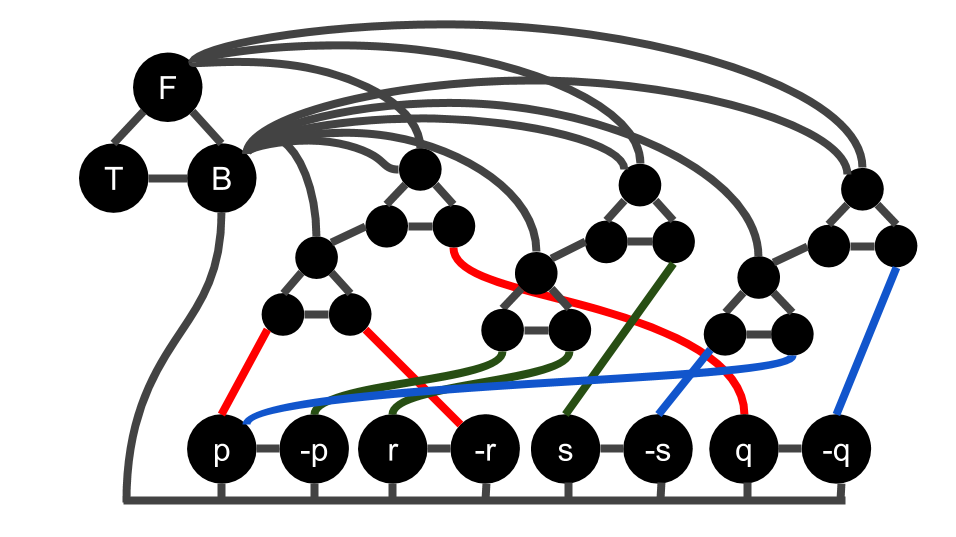
\includegraphics[width=\textwidth]{graph.png}
The above graph is created with three widgets, an $OR$ dual-widget for each clause, a palette widget with $T,F,Base$, and a binary widget for each variable. In the above rendering, a different color is used for each clausal connection set for clarity.

\vspace{2mm} {\bf (b)} \ Write an ASP to solve 3-GC for the resulting graph in (a). \hfill [2 points]\\
Run it with DLV and (clearly explaining) obtain  from it an answer about the colorability of $G(\varphi)$ and the satisfiability of $\varphi$.  Attach \underline{as an appendix} the run with DLV (which implies that the main aspects of the solution should be shown in the main body of the submission). \hfill [5 points]\\

\vspace{2mm} \noindent {\bf Solution (b):}\\
Using $node(\cdot)$ and $edge(\cdot, \cdot)$, we define each node in our graph as a fact and specify the connection. Then we can use a guess-constraint method to narrow down our stable models.
$$col(Node, red) \vee col(Node, green) \vee col(Node, blue) :- node(Node).$$
The above establishes that a node can be one of three colors. A $Node$ is any (every) node that is in the graph. The colors are chosen arbitrarily.
$$:- edge(Node1, Node2),col(Node1, Color), col(Node2, Color).$$
Then we establish a constraint (requirement) that removes solutions with edges that have the same color. This allows us to have a number of stable models as solutions.\\


\noindent {\bf (c)} \ Write an ASP that solves the instance of SAT in (a), directly,  without the detour through 3-GC. The methodology should be general, not a hack for this particular instance. So, explain in what sense it is general. \hfill
[3 points]. \\

\vspace{2mm} \noindent {\bf Solution (c):}\\
Our method will be as such. We will define each variable and its negation:
$$\{pos(p), pos(r), pos(s), ... neg(\neg p), neg(\neg r), neg(\neg s)...\}$$
Then we define a relationship between each pair of variables. Let's call this $boolean(\cdot, \cdot)$. For example:
$$\{boolean(p, \neg p), boolean(r, \neg r)...\}$$
Lastly, for our facts, we define a predicate $clause(\cdot, \cdot ...)$ which has argument length equal to the size of our clauses. We define each clause within our database of facts. In this case, we have only three.\\
To generate our possible answers, we can use the assignments:
$$assign(Var, true) \vee assign(Var, false):- var(Var).$$
$$assign(Var, true) \vee assign(Var, false):- neg(Var).$$
This allows a variable to be either true or false within a model. Next, we have eight constraints in the form:
\begin{equation*}
  \begin{aligned}
:- clause(Var1, Var2, Var3), assign(Var1, false), assign(Var2, false),\\ assign(Var3, false), pos(Var1), pos(Var2), pos(Var3).
\end{aligned}
\end{equation*}

The above constraint omits clauses that have each variable as false, in each of the eight permutations of variable assignments. Lastly, we have the two constraints:
$$:- boolean(Var1, Var2), assign(Var1, true), assign(Var2, true).$$
$$:- boolean(Var1, Var2), assign(Var1, false), assign(Var2, false).$$
These omit the assignment of a variable to both true and false at the same time. We can't have any solutions where any variable and its negation exist.

\vspace{2mm} \noindent {\bf (d)} \ Run the program in (c) on DLV, and give the solution to the decision problem accordingly. Also, obtain the answer sets (models) of the program and explain how you interpret them. Attach the run \underline{as an appendix} (which implies that the main aspects of the solution should be shown in the main body of the submission). \hfill [5 points]

\vspace{2mm} \noindent {\bf Solution (d):}\\
Attached in the appendices is the stable models outputted by this ASP. An example of a satisfying solution is:
\begin{equation*}
  \begin{aligned}
    \{assign(p,true), assign(q,true), assign(r,true), assign(s, true),\\
    assign(np,false), assign(nq,false), assign(nr,false), assign(ns,false)\}
  \end{aligned}
\end{equation*}
We have some redundant information here, with the negated variables, but the assignment is completely valid. There are many other valid models included in the appendices.\\
If we were to apply the assignments to our 3CNF, we could evaluate the formula to true, as each clause would evaluate to true.
\newpage \hspace*{7cm}{\bf \large Appendices}

\vspace{0.5cm}

\noindent {\bf 2b. Trace of Prolog:}
\begin{verbatim}
[trace]  ?- v2.
   Call: (8) v2 ? creep
   Call: (9) v(_2638, _2640) ? creep
^  Call: (10) findall({_2628, _2630},  (r(_2628, _2630), not(s(_2630, _2652))), _2674) ? creep
   Call: (16) r(_2628, _2630) ? creep
   Exit: (16) r(a, b) ? creep
^  Call: (16) not(s(b, _2652)) ? creep
   Call: (17) s(b, _2652) ? creep
   Fail: (17) s(b, _2652) ? creep
^  Exit: (16) not(user:s(b, _2652)) ? creep
   Redo: (16) r(_2628, _2630) ? creep
   Exit: (16) r(a, c) ? creep
^  Call: (16) not(s(c, _2652)) ? creep
   Call: (17) s(c, _2652) ? creep
   Exit: (17) s(c, b) ? creep
^  Fail: (16) not(user:s(c, _2652)) ? creep
   Redo: (16) r(_2628, _2630) ? creep
   Exit: (16) r(c, b) ? creep
^  Call: (16) not(s(b, _2652)) ? creep
   Call: (17) s(b, _2652) ? creep
   Fail: (17) s(b, _2652) ? creep
^  Exit: (16) not(user:s(b, _2652)) ? creep
   Redo: (16) r(_2628, _2630) ? creep
   Exit: (16) r(d, e) ? creep
^  Call: (16) not(s(e, _2652)) ? creep
   Call: (17) s(e, _2652) ? creep
   Fail: (17) s(e, _2652) ? creep
^  Exit: (16) not(user:s(e, _2652)) ? creep
^  Exit: (10) findall({_2628, _2630}, user:(r(_2628, _2630), not(s(_2630, _2652))), [{a, b}, {c, b}, {d, e}]) ? creep
   Exit: (9) v(_2752, [{a, b}, {c, b}, {d, e}]) ? creep
   Call: (9) length([{a, b}, {c, b}, {d, e}], _2754) ? creep
   Exit: (9) length([{a, b}, {c, b}, {d, e}], 3) ? creep
   Call: (9) 3>0 ? creep
   Exit: (9) 3>0 ? creep
   Exit: (8) v2 ? creep
true.
\end{verbatim}
\newpage
\noindent {\bf 5b. Stable Models of 3-Coloring (Limited to 5 models):}
\begin{verbatim}
DLV [build BEN/Dec 17 2012   gcc 4.6.1]

Copyright 1996-2011 Nicola Leone, Gerald Pfeifer, and Wolfgang Faber.
This software is free for academic and non-commercial educational use,
as well as for use by non-profit organisations.
For further information (including commercial use and evaluation licenses)
please contact leone@unical.it, gerald@pfeifer.com, and wf@wfaber.com.

Reading "3col.dl"

{col(f,red), col(t,green), col(b,blue), col(p,red), col(np,green),
col(r,green), col(nr,red), col(s,red), col(ns,green), col(q,green),
col(nq,red), col(c11,green), col(c12,red), col(c13,blue), col(c14,blue),
col(c15,green), col(c16,red), col(c21,blue), col(c22,green), col(c23,red),
col(c24,red), col(c25,green), col(c26,blue), col(c31,red), col(c32,green),
col(c33,blue), col(c34,red), col(c35,green), col(c36,blue)}

{col(f,red), col(t,green), col(b,blue), col(p,red), col(np,green), col(r,red),
col(nr,green), col(s,red), col(ns,green), col(q,green), col(nq,red),
col(c11,green), col(c12,red), col(c13,blue), col(c14,blue), col(c15,green),
col(c16,red), col(c21,red), col(c22,green), col(c23,blue), col(c24,red),
col(c25,green), col(c26,blue), col(c31,red), col(c32,green), col(c33,blue),
col(c34,red), col(c35,green), col(c36,blue)}

{col(f,red), col(t,green), col(b,blue), col(p,red), col(np,green),
col(r,green), col(nr,red), col(s,red), col(ns,green), col(q,green),
col(nq,red), col(c11,green), col(c12,red), col(c13,blue), col(c14,blue),
col(c15,green), col(c16,red), col(c21,red), col(c22,green), col(c23,blue),
col(c24,red), col(c25,green), col(c26,blue), col(c31,red), col(c32,green),
col(c33,blue), col(c34,red), col(c35,green), col(c36,blue)}

{col(f,red), col(t,green), col(b,blue), col(p,red), col(np,green),
col(r,red),col(nr,green), col(s,green), col(ns,red), col(q,red),
col(nq,green), col(c11,blue), col(c12,green), col(c13,red), col(c14,red),
col(c15,green), col(c16,blue), col(c21,blue), col(c22,red), col(c23,green),
col(c24,blue), col(c25,green), col(c26,red), col(c31,blue), col(c32,red),
col(c33,green), col(c34,blue), col(c35,green), col(c36,red)}

{col(f,red), col(t,green), col(b,blue), col(p,red), col(np,green), col(r,red),
col(nr,green), col(s,green), col(ns,red), col(q,red), col(nq,green),
col(c11,blue), col(c12,green), col(c13,red), col(c14,red), col(c15,green),
col(c16,blue), col(c21,red), col(c22,green), col(c23,blue), col(c24,blue),
col(c25,green), col(c26,red), col(c31,blue), col(c32,red), col(c33,green),
col(c34,blue), col(c35,green), col(c36,red)}

\end{verbatim}

\newpage
\noindent {\bf 5d. Stable Models of 3-SAT (Limited to 10 models):}
\begin{verbatim}
DLV [build BEN/Dec 17 2012   gcc 4.6.1]

Copyright 1996-2011 Nicola Leone, Gerald Pfeifer, and Wolfgang Faber.
This software is free for academic and non-commercial educational use,
as well as for use by non-profit organisations.
For further information (including commercial use and evaluation licenses)
please contact leone@unical.it, gerald@pfeifer.com, and wf@wfaber.com.

Reading "3sat.dl"

{assign(p,true), assign(q,true), assign(r,true), assign(s,true),
assign(np,false), assign(nq,false), assign(nr,false), assign(ns,false)}

{assign(p,true), assign(q,false), assign(r,true), assign(s,true),
assign(np,false), assign(nq,true), assign(nr,false), assign(ns,false)}

{assign(p,true), assign(q,true), assign(r,false), assign(s,true),
assign(np,false), assign(nq,false), assign(nr,true), assign(ns,false)}

{assign(p,true), assign(q,false), assign(r,false), assign(s,true),
assign(np,false), assign(nq,true), assign(nr,true), assign(ns,false)}

{assign(p,true), assign(q,true), assign(r,true), assign(s,false),
assign(np,false), assign(nq,false), assign(nr,false), assign(ns,true)}

{assign(p,true), assign(q,false), assign(r,true), assign(s,false),
assign(np,false), assign(nq,true), assign(nr,false), assign(ns,true)}

{assign(p,true), assign(q,true), assign(r,false), assign(s,false),
assign(np,false), assign(nq,false), assign(nr,true), assign(ns,true)}

{assign(p,true), assign(q,false), assign(r,false), assign(s,false),
assign(np,false), assign(nq,true), assign(nr,true), assign(ns,true)}

{assign(p,false), assign(q,true), assign(r,false), assign(s,true),
assign(np,true), assign(nq,false), assign(nr,true), assign(ns,false)}

{assign(p,false), assign(q,false), assign(r,true), assign(s,true),
assign(np,true), assign(nq,true), assign(nr,false), assign(ns,false)}

\end{verbatim}
\newpage
\noindent {\bf 2. Full Definitions For Prolog:}
\begin{verbatim}
r(a, b).
r(a, c).
r(c, a).

s(a, b).
s(a, c).
s(c, b).
s(d, a).

v(_, L):- findall({X,Y},(r(X,Y), not(s(Y,_))),L).
violated :- v(_, L), length(L, X), X>0.

sr(L) :- findall({Y,X}, (r(X,Y), not(r(Y,X)));r(Y,X), L).
\end{verbatim}
\noindent {\bf 5. Full Definitions For 3-Coloring:}
\begin{verbatim}
node(f).
node(t).
node(b).
node(p).
node(np).
node(r).
node(nr).
node(r).
node(nr).
node(s).
node(ns).
node(q).
node(nq).

% or widgets for each clause {c1...c3}
node(c11).
node(c12).
node(c13).
node(c14).
node(c15).
node(c16).

node(c21).
node(c22).
node(c23).
node(c24).
node(c25).
node(c26).

node(c31).
node(c32).
node(c33).
node(c34).
node(c35).
node(c36).

edge(c11, c12).
edge(c12, c13).
edge(c13, c11).
edge(c12, c14).
edge(c14, c15).
edge(c15, c16).
edge(c16, c14).

edge(c21, c22).
edge(c22, c23).
edge(c23, c21).
edge(c22, c24).
edge(c24, c25).
edge(c25, c26).
edge(c26, c24).

edge(c31, c32).
edge(c32, c33).
edge(c33, c31).
edge(c32, c34).
edge(c34, c35).
edge(c35, c36).
edge(c36, c34).

% palette widget
edge(t, f).
edge(t, b).
edge(f, b).

% binary widgets
edge(p, np).
edge(r, nr).
edge(s, ns).
edge(q, nq).

edge(b, p).
edge(b, np).
edge(b, r).
edge(b, nr).
edge(b, s).
edge(b, ns).
edge(b, q).
edge(b, nq).
edge(b, c12).
edge(b, c15).
edge(b, c22).
edge(b, c25).
edge(b, c32).
edge(b, c35).

edge(f, c15).
edge(f, c25).
edge(f, c35).

% CNF mapping below
edge(c11, p).
edge(c13, nr).
edge(c16, q).
edge(c21, np).
edge(c23, r).
edge(c26, s).
edge(c31, ns).
edge(c33, p).
edge(c36, nq).


% GUESS AND CHECK
col(Node, red) v col(Node, green) v col(Node, blue) :- node(Node).
% CONSTRAINT
:- edge(Node1, Node2),
   col(Node1, Color), col(Node2, Color).
\end{verbatim}
\newpage
\noindent {\bf 5. Full Definitions For 3-SAT:}
\begin{verbatim}
pos(p).
pos(q).
pos(r).
pos(s).
neg(np).
neg(nq).
neg(nr).
neg(ns).

clause(p, nr, q).
clause(np, r, s).
clause(ns, p, nq).

boolean(p, np).
boolean(q, nq).
boolean(r, nr).
boolean(s, ns).

% GUESS AND CHECK
assign(Var, true) v assign(Var, false):- pos(Var).
assign(Var, true) v assign(Var, false):- neg(Var).
% CONSTRAINT
:- clause(Var1, Var2, Var3), assign(Var1, false), assign(Var2, false),
assign(Var3, false), pos(Var1), pos(Var2), pos(Var3).
:- clause(Var1, Var2, Var3), assign(Var1, false), assign(Var2, false),
assign(Var3, true), pos(Var1), pos(Var2), neg(Var3).
:- clause(Var1, Var2, Var3), assign(Var1, false), assign(Var2, true),
assign(Var3, false), pos(Var1), neg(Var2), pos(Var3).
:- clause(Var1, Var2, Var3), assign(Var1, true), assign(Var2, false),
assign(Var3, false), neg(Var1), pos(Var2), pos(Var3).
:- clause(Var1, Var2, Var3), assign(Var1, false), assign(Var2, true),
assign(Var3, true), pos(Var1), neg(Var2), neg(Var3).
:- clause(Var1, Var2, Var3), assign(Var1, true), assign(Var2, false),
assign(Var3, true), neg(Var1), pos(Var2), neg(Var3).
:- clause(Var1, Var2, Var3), assign(Var1, true), assign(Var2, true),
assign(Var3, false), neg(Var1), neg(Var2), pos(Var3).
:- clause(Var1, Var2, Var3), assign(Var1, true), assign(Var2, true),
assign(Var3, true), neg(Var1), neg(Var2), neg(Var3).
:- boolean(Var1, Var2), assign(Var1, true), assign(Var2, true).
:- boolean(Var1, Var2), assign(Var1, false), assign(Var2, false).
\end{verbatim}
\end{document} 